\documentclass[10pt]{article}

% Packages
\usepackage{graphicx}
\usepackage{amsmath}
\usepackage{hyperref}
\usepackage{geometry}
\usepackage{changepage}
\usepackage{fancyhdr}
\usepackage{tocloft}
\usepackage{titlesec}
\usepackage{lastpage}
\usepackage{caption}
\usepackage{tabularx}
\usepackage{array}
\usepackage{multicol}

\captionsetup[figure]{
    font={it, small},
    labelfont=bf,
    labelsep=period,
    justification=centering,
    singlelinecheck=false
}

\captionsetup[table]{
    font={it, small},
    labelfont=bf,
    labelsep=period,
    justification=centering,
    singlelinecheck=false
}

\titleformat{\section}
{\normalsize\bfseries}
{\thesection \, \textbar}
{0.5em}
{}

\titleformat{\subsection}
{\normalsize\bfseries}
{\thesubsection \, \textbar}
{0.5em}
{}

\geometry{a4paper, margin=1in}

\fancyhf{}
\fancyfoot[L]{
    \scriptsize\bfseries
    Department of Computer Engineering\\
    Chulalongkorn University
}

\renewcommand{\headrulewidth}{0pt}
\renewcommand{\footrulewidth}{0.5pt}
\renewcommand{\cftsecaftersnum}{.}

\begin{document}

    \begin{titlepage}
        \noindent
{\footnotesize
Computer Engineering Capstone Project Proposal
\par}

\vspace{0.3cm}

\noindent
{\Large\bfseries
Utilization of High Precision Software System
\par}

\noindent
{\Large\bfseries
for Development of Interactive Entertainment Media
\par}

\vspace{0.4cm}

\noindent
{\small
Tapaneeya Odmung   \, \textbar \,
Wachirawich Kanil  \, \textbar \,
Pranesh Ingkanunt  \, \textbar \,
Rangsiman Jearuksa
\par}

\vspace{0.3cm}

\noindent
{\scriptsize
Department of Computer Engineering, Chulalongkorn University, Bangkok, Thailand
\par}

\vspace{0.3cm}

\noindent
{\scriptsize
\textbf{Advisor:}
Asst. Prof. Vishnu Kotrajaras (vishnu@cp.eng.chula.ac.th),
Kamin Kolyutsakul (something@somewhere.com)
\par}

\vspace{0.3cm}

\noindent
{\scriptsize
\textbf{Keywords:}
high-performance computing,
computer graphics,
real-time rendering,
parallel processing,
software architecture,
game engine
\par}

\vspace{0.3cm}

\noindent
{\normalsize \today \par}

\vspace{0.5cm}

\begin{center}
    \includegraphics[width=\textwidth, keepaspectratio]{images/title}
\end{center}

%{\rule{\textwidth}{0.5px}\par}
%\vspace{-0.4cm}
        \noindent
        {\rule{\textwidth}{0.5px}\par}
        \vspace{-0.4cm}
        \begin{adjustwidth}{0.5cm}{0.5cm}
    \section*{\normalsize Abstract}
    \vspace{-0.3cm}
    \normalsize
    This project focuses on addressing the lack of a versatile and high-performance general purpose interactive media
    creation framework, which is important due to the prevalence of interactive media in academic and medical contexts.
    The objectives of this project are to analyze the limitations of existing game engine architectures, particularly
    in their usage of creating general purpose interactive media, as well as to explore alternative paradigms and
    finally develop a framework that can streamline its creation with minimal development costs and maintaining high
    performance and usability across various domains.
    To achieve these objectives, the proposed solution involves an operating-system-like game engine, integrating
    the Entity-Component-Structure framework with operating systems concepts, while utilizing aggressive C++ compile-time
    optimization to increase performance.
    \\\\
    The methodology will include C++20, DirectX 11, and Windows API to design and analyze the system, and
    GoogleTest to validate it.
    The outcomes we expected from this project are a proposal, a deliverable prototype, and a system documentation,
    which we expected will provide industrial benefits to future creations of interactive media.
    \\\\
    \textbf{Keywords:} Entity-Component-System, Game Design, Optimization, C++

\end{adjustwidth}
        \noindent
        {\rule{\textwidth}{0.5px}\par}
    \end{titlepage}

    \pagestyle{fancy}
    \pagenumbering{roman}
    \fancyfoot[R]{\thepage}

    \tableofcontents
    \addcontentsline{toc}{section}{Contents}
    \thispagestyle{fancy}
    \newpage

    \fancyfoot[R]{
        \thepage\ of \pageref{subsec:intellectual-property-and-law}
    }
    \pagenumbering{arabic}
    \setcounter{page}{1}
    \twocolumn

    \section{Introduction}
\label{sec:introduction}
In recent years, interactive media is found in various places throughout digital society,
such as within games, visual effects in movies, applications, or Visual Reality (VR)
with usage covering many fields.
For example, Virtual Reality as a recovery tool in a medical system.
Because of this demand, the performance requirements are becoming more prominent.
But on the hardware side, the growth of performance
is far less than the demand.
\\\\
The current trend of creating interactive media is using game engines such as Unity, Godot, or
Unreal to create this type of media.
But these systems weren't built with this general usage in mind, but rather were specialized for creating games.
Because of this, these engines might not be suitable for widespread everyday usage with such high demands.
Many companies decided to write their own systems from the ground up, which led to slower development while accruing
unnecessary costs.
\\\\
These situations raise the question — whether it is possible to create a system that can be used to generate such media
and highly optimal for various tasks while also remaining highly optimized.
\\\\
To test the precision of such software, a good test is to create a rhythm game.
This type of media is forced to have high-precision inputs to provide good responsiveness to
the user and make a better impression on them.
To prove the generality of the system, a bullet hell mechanic is added to the game to showcase seamless
integration between the two highly different logics.
Lastly, to check if the system is viable from a business standpoint, we will develop this game
to compete in the Game Talent Showcase by Thailand Game Association (TGA).

\subsection{Background}
\label{subsec:background}
% Background goes here

\subsubsection*{Entity-Component-System Architecture}

Entity-component-system (ECS) is a software architectural pattern mostly used in game development.
Its mechanisms are characterized by the entities, composed of components of data,
and the systems which operate upon those components.
The behaviors of these entities are modified at runtime by systems modifying, adding, or removing the components
attached to said entities.
\\\\
Implementations of ECS already exist, even in production contexts.
One of the more popular implementations is EnTT~\cite{ValtoLibraries_EnTT}, a header-only C++ library for game programming.
This library has been used to develop many game titles, the most major of which is Minecraft.
Another popular implementation is Bevy ECS~\cite{Bevy_Engine}, a data-driven game engine built in Rust.
\\\\
However, most existing ECS libraries use runtime component registration, perform type-erased iteration, or resolve
system dependencies at runtime, or some combination of the above.
While they often optimize queries via template views or code specialization, they cannot fully eliminate
runtime overhead associated with registration, lookup, or caching.
Experimental systems like Vittorio's ECST~\cite{vittorio} achieve deep compile-time specialization
but are not production-ready due to ambiguity in naming, sparse documentation, and hidden dependencies.
\\\\
We want to combine the best of both worlds — to create an ECS framework that registers and determines component types
and system dependencies at compile-time, while ensuring code flexibility and production-ready performance, complete
with rigorous documentation.

\subsubsection*{Market Research}

The computer software market has been growing for many years, and software performance continues to develop 
as the demand for advanced software systems increases in various industries.
We have looked into a report of the High Performance Computing Software Market~\cite{HPC_Software_Market_Research} to
understand the possible trend of software engineering in the future.
According to the research, the market is forecasted to grow from 45.5 billion USD in 2024 to 99 billion USD by 2035.
\\\\
High performance computing (HPC) software has become essential for optimizing complex processes to ensure high-speed operations.
With the increased use of advanced technology, including artificial intelligence, machine learning, simulations, and many more 
modules and services, HPC software is necessary for these technologies to function properly.
Additionally, organizations and companies are also interested in software efficiency to lower the costs of computing resources, 
and implementation with cloud services.
This can be marked as another direction of the market which focuses on sustainable and energy-efficient products.
Therefore, an ideal software system for the industry should be able to provide high performance while simultaneously being 
optimized and efficient to reduce operation costs and resources.
\\\\
Upon considering regional valuation, North America is the leader of the global HPC market, valued at 20.0 billion USD in 2024, 
with the U.S.A. being the key driver of the market due to strong demand for highly advanced software and contributions from 
various tech companies, including Microsoft, IBM, AWS, and NVIDIA.
Following North America is Europe, with a valuation of 11.0 billion USD in 2024, and Asia-Pacific region (APAC), valued at 
10.0 billion USD in 2024.
The global market trend shows that many countries around the world are investing in HPC software and companies are innovating 
new technologies to capitalize on the growing demands.
\\\\
Our project does not cover only the development of high-performance software, but also its utilization.
Therefore, we decided to research a performance-reliant medium for computer software: video games.
We have looked into a report of Gaming Software Market Analysis 2025-2029~\cite{Gaming_Software_Market_Analysis} to understand the direction of 
the gaming industry in different regions.
The market has been growing significantly due to advancements in game engines which support mobile and tablet games, along with 
increasing popularity in eSports, short for electronic sports, which is a form of competition using video games, creating new 
revenue streams for the market.
Game engines are being optimized to improve performance and graphical processes. To capitalize on market opportunities, gaming 
software companies must keep up in research and development of technologies to provide new experiences to consumers.
\\\\
According to Technavio’s analysts, the Asia Pacific (APAC) region is estimated to contribute 43\% to the growth of the global 
market during the forecast period.
With China, Japan, and India as leading countries, APAC dominates the market due to the largest number of mobile gamers, 
in addition to the increase in smartphone usage and high-speed internet services.
The advancements in game engines serve as the primary driver for the rise of the gaming software market, driven by the 
evolution of technologies in rendering, animation, graphics, augmented/virtual reality (AR/VR), and artificial intelligence (AI).
Game development tools, including engines, continue to be a crucial investment for businesses in the industry.

\subsection{Problem Statement}
\label{subsec:problem-statement}

\subsection{Objectives}
\label{subsec:objectives}

\subsection{Scope \& Limitations}
\label{subsec:scope-and-limitation}

\subsection{Expected Benefits}
\label{subsec:expected-benefits}
    \section{Problem Solving \& Related Work}
\label{sec:problem-solving-related-work}

\subsection{Review of Existing Knowledge}
\label{subsec:review-of-existing-knowledge}

\subsubsection*{Software Bloat Analysis}

As hardware has been improving with microprocessors since the 1980s, software engineering practices have
also evolved to match the higher performance provided by the runtime system and architecture.
However, the growth of software requirements proves to be higher in terms of functionality and size.
As the software complexity rapidly increases, the performance improvement from hardware has not been 
able to grow fast enough to satisfy the demands.
Hence, performance optimization is necessary in modern software despite the advancement of CPUs and 
memory systems.
\\\\
A study on software bloat~\cite{Software_Bloat_Analysis} claimed that the main cause of performance 
problems in software systems was not from hardware limitations, but from lack of optimization in software design.
Modern object-oriented applications often suffer from inefficient use of memory, such as memory leaks 
which accumulate unused objects and exhaust the heap space, and algorithms that are not suitable for 
large data sets.
Though multicore processors have been widely adapted to improve performance via parallelism, the root
causes of performance bottlenecks are left unsolved.
\\\\
Solving performance issues in software systems requires effort, time, and knowledge to analyze and 
pinpoint the causes of bottlenecks.
Though there are studies on bloat detection and analysis to identify the sources of inefficiencies 
in software systems, there are still challenges in the process of bloat removal.
Because the definition of bloat is subjective and varies across different applications, it is challenging
to create a universal solution for bloat removal.
Therefore, the process of removing performance bottlenecks requires careful consideration and specification 
to precisely resolve the issues without affecting the intended functionality of the software.

\subsubsection*{Entity-Component-System Architecture}

Entity-component-system (ECS) is a software architectural pattern mostly used in game development.
Its mechanisms are characterized by the entities, composed of components of data,
and the systems which operate upon those components.
The behaviors of these entities are modified at runtime by systems modifying, adding, or removing the components
attached to said entities.
\\\\
Implementations of ECS already exist, even in production contexts.
One of the more popular implementations is EnTT~\cite{ValtoLibraries_EnTT}, a header-only C++ library for game programming.
This library has been used to develop many game titles, the most major of which is Minecraft.
Another popular implementation is Bevy ECS~\cite{Bevy_Engine}, a data-driven game engine built in Rust.
\\\\
However, most existing ECS libraries use runtime component registration, perform type-erased iteration, or resolve
system dependencies at runtime, or some combination of the above.
While they often optimize queries via template views or code specialization, they cannot fully eliminate
runtime overhead associated with registration, lookup, or caching.
Experimental systems like Vittorio's ECST~\cite{vittorio} achieve deep compile-time specialization
but are not production-ready due to ambiguity in naming, sparse documentation, and hidden dependencies.

\subsection{Comparison with Existing Systems}
\label{subsec:comparison-with-existing-systems}

We have reviewed existing well-known free software systems that are designed for interactive media
development to understand their strengths and weaknesses in their architectures and design.

\subsubsection*{Game Engines}

When comparing current popular game engines, such as Unity~\cite{Unity_Engine} and Unreal Engine~\cite{Unreal_Engine}, 
there are some notable differences in their architecture and performance.
\\\\
Unity uses a component-based architecture, where game objects can contain various components which 
determine their behaviors.
This architecture allows for flexibility and modularity, as components can be added or removed dynamically 
from objects.
Unity also provides a data-oriented technology stack (DOTS)~\cite{Unity_DOTS} that utilizes
ECS architecture to improve performance by optimizing memory layout and enabling multithreading on 
multiple packages.
The system is built on a native C / C++ engine core, reducing runtime overhead and allowing
cross-platform compatibility.
However, the system uses C\# on .NET Framework for the scripting layer, which introduces memory management
overhead from frequent garbage collection cycles.
Additionally, Unity's architecture relies on object-oriented programming (OOP), which can lead to performance 
bottlenecks when managing large numbers of game objects due to deep inheritance hierarchies.
This, along with tight coupling between game objects and their behaviors, leads to challenges in scalability and maintainability.
\\\\
Unreal Engine also uses a similar component-based architecture, with objects composed of various components 
to define their behaviors, but the engine is built entirely in C++, allowing for high 
performance and low-level control over system resources.
The engine is also built with modular subsystems (rendering, physics, audio, etc.) that utilize multithreading 
to improve performance.
Unreal Engine 5 introduces a new framework similar to ECS called MassEntity~\cite{Unreal_MassEntity}, which aims to 
improve performance by optimizing memory layout for large-scale simulations.
Currently, in 2025, the MassEntity system is still in development and not fully integrated into the engine.
On the other hand, the engine uses a visual scripting system called Blueprints, which can introduce additional 
performance overhead.
Moreover, Unreal Engine contains advanced features such as real-time ray tracing and high-fidelity graphics, 
which can be resource-intensive and may require high-end hardware to run smoothly.
\\\\
Upon comparison, both engines have their strengths and weaknesses in terms of architecture and performance, 
which can impact their suitability for different types of projects.
Both engines utilize component-based architectures that promote modularity and flexibility.
Unity's flexibility and modularity make it a good choice for smaller projects or those requiring rapid 
developing cycles, but could suffer from performance issues in larger-scale applications.
Meanwhile, Unreal Engine's high performance and advanced features aim for high-quality
3D projects, but the system is not built to support the general media applications due to its massive 
performance costs.

\subsubsection*{Digital Content Creation Tools}

Digital Content Creation (DCC) tools, such as Blender~\cite{Blender}, are widely used in the creation 
of 3D models, animations, and visual effects.
\\\\
Blender is an open-source DCC tool built with native C/C++ core for optimized data processing and 
memory management.
The system uses dependency graphs~\cite{Blender_Dependency} to update and manage relationships of scene data
efficiently by only considering what is dependent on the modified value.
Blender also uses a specialized system called DNA~\cite{Blender_DNA} and RNA~\cite{Blender_RNA} to manage 
data structures and properties.
DNA is a low-level system that defines the data structures used in Blender to enable forward and backward 
compatibility across different versions of the software.
The system generates a binary representation for the data structures, called Structure DNA (SDNA).
Then, SDNA is embedded with the actual data, making the contents in the files self-descriptive and portable 
across other versions of the system.
On top of DNA, RNA is a higher-level system that provides an interface for accessing and manipulating 
Blender's data structures at runtime, allowing for dynamic interaction with the data.
\\\\
Blender's architecture is designed to be modular and extensible from its data-block structure, allowing for
the addition of new features from plugins and scripts.
However, the system uses Python for scripting layer and API which, while flexible and easy to use,
can introduce performance overhead due to its interpreted nature.
Additionally, Blender's DNA/RNA systems can add complexity to the data management process, which may cause 
complications for developers when improving or extending the system in the future.
Therefore, while Blender's architecture is optimized for performance and flexibility, there are still 
challenges in balancing these aspects effectively.

\subsection{Gap Analysis}
\label{subsec:gap-analysis}

Upon reviewing existing systems and related work, it is clear that each system has its own strengths depending
on the intended use cases.
However, there are still gaps and limitations that can be addressed to improve performance and flexibility.
\\\\
Game engines in the past often relied on object-oriented programming (OOP) principles, which make the system easy to 
understand due to its similar concepts to real-world objects.
However, OOP is often denounced in modern software engineering for its complexity and inefficiency in managing 
large-scale applications with numerous data structures.
While concepts like inheritance and polymorphism provide flexibility in development, they can also be overwhelmed 
when managing complex relationships between objects, leading to tight coupling and deep inheritance hierarchies.
Hence, game engines like Unity and Unreal Engine have been shifting towards data-oriented designs like ECS to improve 
performance and scalability.
\\\\
As software demands continue to surpass the current hardware capabilities, system optimization is crucial to ensure 
efficient resource utilization and performance.
A recent study on game engine efficiency~\cite{Game_Engine_Efficiency} experimented with Unity, Unreal Engine, 
Godot~\cite{Godot_Engine}, and a custom-built engine using ECS architecture and scripting system in C syntax.
When using the engines to buid a simple 2D game, the study showed that as the number of objects increased, the custom 
ECS engine outperformed every other engine in terms of CPU usage, power consumption, and memory usage.
This indicates that further optimization is still possible with efficient architecture.

\subsection{Linkage to Project}
\label{subsec:linkage-to-project}

Upon analyzing existing systems in the market, it is evident that there are still gaps and limitations 
that can be addressed to improve performance and flexibility.
We aim to create a framework that combines the strengths of existing architectures while addressing 
their weaknesses.
By utilizing the ECS architecture, we can achieve better performance and scalability compared to
traditional OOP-based designs.
We want to combine the best of both worlds \textemdash to create an ECS framework that registers and determines component types
and system dependencies at compile-time, while ensuring code flexibility and production-ready performance, complete
with rigorous documentation.
\\\\
In order to showcase the capabilities of our proposed framework, we plan to develop a game prototype that utilizes 
the system performance to its fullest potential.
We have designed a game that combines two performance-intensive genres: rhythm games and bullet hell shooters.
Rhythm games require players to interact with the game in sync with the music, demanding precise timing and 
responsiveness as much as in millisecond accuracy.
Bullet hell shooters, on the other hand, involve navigating through a screen filled with numerous projectiles, 
requiring efficient handling of a large number of entities and collision detection.
By merging these two genres, we can create a game that demonstrates our framework's performance and responsiveness.
    \section{System Design}
\label{sec:system-design}

\subsection{System Overview}
\label{subsec:system-overview}

\subsubsection*{Engine Design}

The project's core engine design, as stated before, will use an ECS framework that registers and
determines components and system dependencies at compile-time.
The declaration of a single ECS instance that registers all components and systems would result in
wasteful usage of memory and projected performance decreases due to the large variety of components involved.
As such, we have opted to use multiple smaller ECS instances that each take control of a smaller part of the game.
We refer to these smaller ECS instances, alongside the data necessary to register related components and systems,
as well as compute and store initial data into those instances, as scenes.
Communications between scenes, such as the data transfer when creating a new scene, are facilitated through
a manager, which will also execute the registered systems during the main game loop.
DirectX 11 is used for the rendering of the game with the use of a custom rendering pipeline implementation.
User input is collected through the Windows API\@.

For the actual implementation of these compile-time optimizations, we take advantage of C++'s concept of templates.
By using component and system data types as template parameters, we can use template specialization to let
the compiler generate code specific to our use case.
Since each system is a function, this also means we get usage of functions without relying on indirect calls,
which is a common pain point in engine design.
\\\\
The benefits of template specialization can be seen with a key part of the ECS instance, the resource manager.
The resource manager manages entities along with any components attached to those entities, together referred to as resources.
The resource manager takes a size integer and any number of structures as template parameters and treats those
structures as registered components in this instance.
It will create a resource pool of each registered component with the specified size when constructed, each of
which will reserve their own memory depending on the component's size and the pool size.
By accessing these components through template specialization, code is generated such that the abstraction layers
are removed from the code when compiled.
\\\\
While systems are being run, entities with select component archetypes are iterated upon.
If components are added or removed during iteration, this may invalidate references or otherwise cause unpredictable behavior.
To avoid such hazards, a structure must be created with the purpose to defer all attempts to add or remove components
and to apply such changes after all systems complete execution.
Borrowing the term from operating systems, we refer to this structure with elevated permissions to modify resources
as the syscall.
The syscall must know the components registered to its coupled resource manager so that it can add the appropriate
components.
When systems want to add or remove components from an entity, they make the request to the ECS instance, which
will schedule the changes in its internal syscall.
\\\\
Systems operate upon entities based on whether they fulfill certain component requirements.
For complex systems, the requirements can be rather complex, and entities may be retrieved multiple times
under different requirements.
Some implementations have the ECS instance be provided as a function argument to each system so that entities
can be retrieved directly from internal resources via templated retrieval functions.
We decided, instead, that systems define query data structures as function arguments, which describes the components
that entity references stored within are guaranteed to possess.
When the system is run, the ECS instance will internally fulfill each query requirement by fetching and filtering
from the resource manager before passing them to the system.
This way, the system's implementation does not concern itself with fetching data from the ECS instance.

\subsubsection*{Game Design}

The project's core game design will involve combining rhythm games and bullet hell games into a hybrid game
structured around distinct but smoothly transitioning phases,
thus requiring a seamless transition between the two, creating a revolutionary take on hybrid games.
Considering that both of the games hugely relied on great optimization, as with a little disruption,
it can cause a fatal mistake for the player inciting frustration, the design of the game must be made cautiously.
\\\\
The bullet hell section is mostly composed of large numbers of bullets and particles,
while great performance is still required to retain the player’s fluidity of movement.
To achieve this, an ECS architecture is highly favored as opposed to object-oriented
since the large number of entities can be handled more efficiently with it.
Entities of the system are composed of player, bullets, boss, enemies, background and effects
using shared components such as position, velocity, sprite, shader, etc.
Each system will be executed every frame thus handling the entity movement,
collision check and input allowing it to handle all the bullets in a frame efficiently.
Such systems consist of a player system, movement system, collision system, particle system and much more.
The core mechanics are that, for each frame, the input was processed to control the player system.
Meanwhile, the collision system will check each ongoing colliding entity by computing if each entity with a collider component
is colliding with another entity.
Then, the corresponding function will be triggered to apply change to the state such as the player taking damage and making change to the player’s health UI\@.
Moreover, the movement system computes the next frame position to render, and lastly, the animation system will render the right frame of the animation at the correct time.
\\\\
Rhythm games require precise timing and precision to catch the note at the right time,
so very few optimization issues can be tolerated as a result.
However, ECS architecture is powerful enough to handle all the requirements
such as notes quantities and an accurate time tracking device centralized by a single system.
With entities as simple as notes, lanes and judgment, components are widely adjustable with speed, timing and judgment.
In addition, the system design is fairly simple as the input system and judgment system are centralized
and the note system moves all notes called.
Along with the bullet hell section, they contain backgrounds that are adjustable by shader and particle effects.
The core mechanic revolves around spawning the notes at the right time as set up.
Then, each note will be called by the movement system to calculate the position of the sprite.
However, the real logic of the note is being computed by another system that reduces its timing to be
compared within the judgment system.
Lastly, the judgment system calls the corresponding system to handle whether if the note has been well-time pressed and sending responses to the player.
\\\\
Transitioning between both types of gameplay proves to be a great challenge design-wise.
It has to be smooth and seamless enough to not disrupt the precision-hungry gameplay of both games.
Firstly, in the whole game process, only one game scene may be rendered to minimize time to transition
as the whole scene will be loaded and initiated only once from the start.
If the transition is happening, the gameplay should be frozen and any progress should not be counted during the process,
allowing the player to get ready to adjust their gameplay smoothly.
The transition's animation has to telegraph the player clearly to make them aware that the gameplay is going to be changed
as the timer UI counts down to inform the duration and delay of the transition precisely.
Lastly, the screen changing the gameplay rendered has to be transition creative by splitting the screen in two and slowly expanding the next gameplay.
To achieve this, a line animation system is used to express animation of the transition, and the game transition system
will be triggered if the state has been changed.
Following this, the new gameplay is rendered for a section of the screen expanding until full.
\\\\
The biggest concern of the system is the control of the rhythm game's charts and bullet hell's patterns
needing to be not too exhaustingly difficult to control as both games require vast amounts of complicated pattern and timing design.
A solution proposed would be to create our own scripting language and a corresponding compiler such as a chart file.
Practicing these techniques makes designing and implementing charts and patterns much easier,
allowing more complex and challenging design and features.
\\\\
To complete a game, a narrative device should be implemented to make the game more immersive and enjoyable;
the proposed gameplay would be a 2D side-scrolling style that allows players to choose a level and progress the story of the gameplay.
Additionally, explorations are added to the game such as interacting with an interactable such as NPC, or objects,
getting new in-game items and accessing new areas.
Such requirements must be implemented with an entirely separate system.
Interactable and solid collision components are needed to be implemented along with the new system,
for example, a new movement system, interact system and area load system.
\\\\
Lastly, using ECS, UI entities are being rendered concurrently in a higher priority by default.
The entities will have a position, text, sprite and animation components and are created organizedly using functions for each set of UIs.
For sound and music in the game, just like UIs as each is assigned to its own entity holding a tag or trigger to be played on an instance sound system at the right time.
Finally, the cutscene could be added as a video format to be rendered in an instance video player system.



\subsection{Components}
\label{subsec:components}

The system is a self-contained application, but interfacing with a keyboard and mouse is required for its operation.



\subsection{Constraints Considered}
\label{subsec:constraints-considered}

Due to the usage of the Windows API and DirectX 11, the system is to be operated and published only on
the Windows operating system.

\subsection{Diagrams}
\label{subsec:diagrams}

\vspace{0.5cm}

\noindent
\begin{minipage}{\columnwidth}
    \centering
    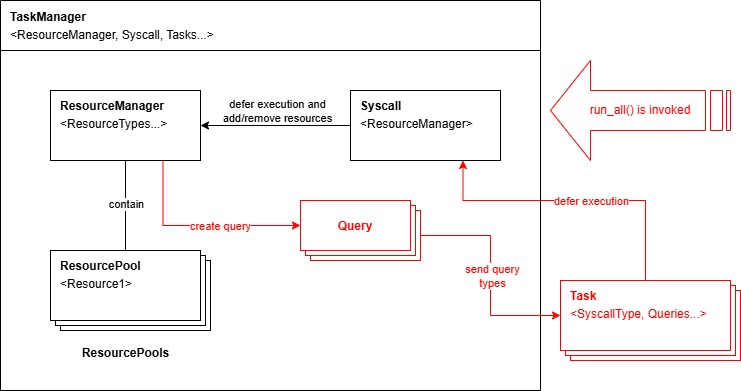
\includegraphics[width=\columnwidth, keepaspectratio]{images/taskmanager}
    \captionof{figure}{A diagram showing how task manager works}
    \label{fig:taskmanager}
\end{minipage}

\vspace{0.5cm}

\noindent Figure~\ref{fig:taskmanager} shows the composition of the task manager, a unit of ECS instance.
Using template instantiation, the task manager knows the type of its resources(components) and tasks(systems)
and creates the required storage and functionality when constructed.
When the task manager receives a signal to advance its state, depending on the type of task, it will
formulate the appropriate queried resource data structure and apply it as a parameter to its registered tasks.
The tasks state the query requirements in advance so that this process can be inferred at compile-time.

\vspace{0.5cm}

\noindent
\begin{minipage}{\columnwidth}
    \centering
    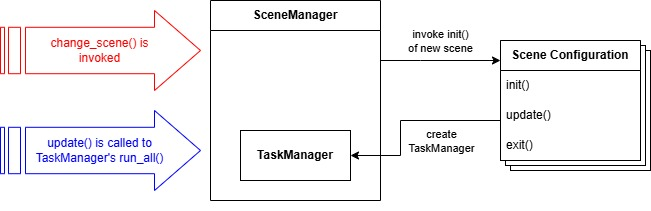
\includegraphics[width=\columnwidth, keepaspectratio]{images/scenemanager}
    \captionof{figure}{A diagram showing how scene manager works}
    \label{fig:scenemanager}
\end{minipage}

\vspace{0.5cm}

\noindent Figure~\ref{fig:scenemanager} shows the composition of the scene manager, which manages ECS instances.
The scene manager registers a collection of scenes in advance, where each scene is a data structure with the
functions to create a task manager instance.
When the scene manager chooses a scene to change to, the scene's functions are invoked, returning the created
task manager instance to the scene manager to update during the game loop.

\vspace{0.5cm}

\noindent
\begin{minipage}{\columnwidth}
    \centering
    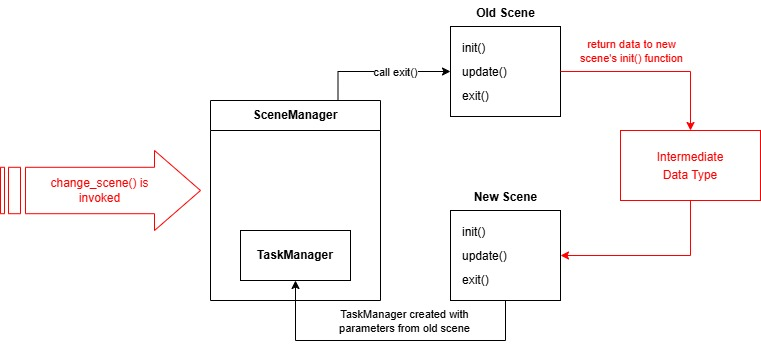
\includegraphics[width=\columnwidth, keepaspectratio]{images/scenemanager2}
    \captionof{figure}{A diagram showing how scene manager transfers data from old scene to new scene}
    \label{fig:scenemanager2}
\end{minipage}

\vspace{0.5cm}

\noindent When the game logic leaves one scene and enters another, persistent data between scenes may be required.
The operation of this data transfer is shown in Figure~\ref{fig:scenemanager2}.
As shown, when a scene is exited, it returns an intermediate data structure containing the data of resources
it wishes to transfer to the next scene.
This data structure is then applied as arguments for initialization of the scene to enter.
\\\\
Through the functionality of the task manager and scene manager, the assembly and disassembly of memory-efficient
ECS instances with complete knowledge of required data types can be achieved without losing any functionality of
single-instance ECS implementations.

\vspace{0.5cm}

\noindent
\begin{minipage}{\columnwidth}
    \centering
    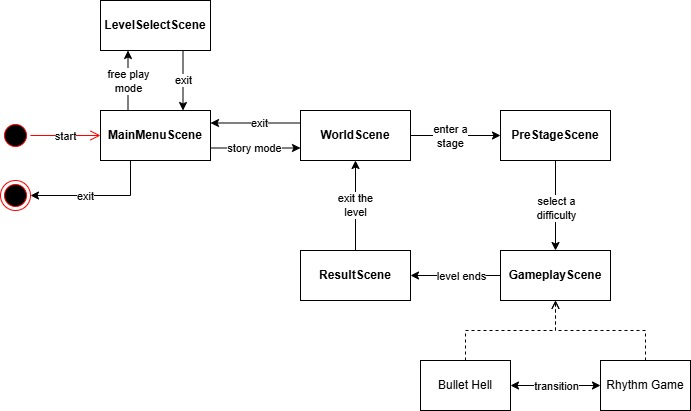
\includegraphics[width=\columnwidth, keepaspectratio]{images/gameflow}
    \captionof{figure}{A diagram showing scene flow of the game prototype}
    \label{fig:gameflow}
\end{minipage}

\vspace{0.5cm}

\noindent Figure~\ref{fig:gameflow} shows how the scenes in our game should flow.
The game starts from the main menu scene where the player can choose to enter the game or exit.
After the player chooses to enter the game, the game's world scene will be loaded.
There will be objects across the world that act as stages that the player can interact with to
enter the level.
When the player interacts with a stage object, the game will transition to a pre-stage scene, where
they can select which instrument to use in the level.
Each instrument represents a different difficulty level.
The player can choose to start the level with the selected instrument or return to the world.
\\\\
Once the player starts the level, the game will transition to the main gameplay scene.
The gameplay scene consists of both bullet hell and rhythm game phases.
In this scene, as the level begins, the player will start with the bullet hell phase.
The player must avoid incoming obstacles from the enemy and survive throughout the phase.
If the player's health reaches zero at any point, the gameplay will end, failing the level.
After surviving for a certain amount of time, the game will transition to the rhythm game phase.
In this phase, the player must hit the notes in time with the music to attack the enemy.
Each successful note hit will slightly fill the enemy's gauge and heal the player, while missed notes will 
only deplete the gauge.
The player must fill the gauge above a certain threshold to defeat the enemy and complete the level.
Then, the game will transition back to the bullet hell phase again.
This cycle continues until the song ends or the player is defeated first.
If the player successfully fills the gauge above the threshold by the end of the song, the player wins.
Otherwise, it is considered a draw.
\\\\
After the gameplay ends, regardless if the player wins, loses or draws, the game will transition to the result
scene, displaying the player's performance statistics.
Then, the player will return to the world scene to continue exploring or choose another level.
    \newpage
    \onecolumn %change into multicolumn
    \section{Teamwork Plan}
\label{sec:teamwork-plan}

\subsection{Roles and Responsibilities}
\label{subsec:roles-and-responsibilities}

\subsection{Collaborative Plan}
\label{subsec:collaborative-plan}

\subsection{Task Coverage}
\label{subsec:task-coverage}

\subsection{Workload Balance}
\label{subsec:workload-balance}
    \twocolumn
    \section{Timeline}
\label{sec:timeline}
    \section{Planned Work}
\label{sec:planned-work}
    \section{Ethic, Privacy, and Professional Consideration}
\label{sec:ethic-privacy-and-professional-consideration}

\subsection{Plagiarism Check}
\label{subsec:plagiarism-check}

\subsection{Credibility of Information}
\label{subsec:credibility-of-information}

The project mostly references the verified official documentation including DirectX and Microsoft C++ documentation,
as well as credible research and articles on engine architecture and game design theory.
All development and design are supported by reliable and recognized sources in software engineering and game development literature,
ensuring grounded and reliable information.

\subsection{Intellectual Property \& Law}
\label{subsec:intellectual-property-and-law}

All codes, tools and assets created during the project are original works owned by the team.
DirectX, Microsoft's window’s APIs, used in this project is free to use without any attribution so long as no binary tampering or falsely acclaimed trademark usage.
No additional third-party libraries or resources are used.
All visual and audio assets will be self-produced.
The project will comply with software licensing terms, and university policies regarding intellectual property and academic integrity.
The team allows reusers to distribute, remix, adapt, and build upon the material in any medium or format for research or noncommercial purposes only,
and only so long as attribution is given to the creator.

    \newpage

    \onecolumn
    \fancyfoot[R]{\thepage}
    \pagenumbering{alph}

    \addcontentsline{toc}{section}{References}
    \bibliographystyle{ieeetr}
    \bibliography{refs}
    \newpage

    % -- Appendix if needed (which you will) -- %
    \appendix
    \renewcommand{\thesection}{\Alph{section}}
    \titleformat{\section}
    {\normalsize\bfseries}
    {Appendix \thesection \, \textbar}
    {0.5em}
    {}

    \makeatletter
    \renewcommand{\listoffigures}{%
        \begingroup
        \let\old@makecaption\@makecaption
        \renewcommand{\@makecaption}[2]{##2\\}%
        \parindent\z@
        \refstepcounter{section}
        \section*{Appendix \thesection \, \textbar \vspace{0.5em} List of Figures}
        \label{sec:appendix-list-of-figures}
        \addcontentsline{toc}{section}{Appendix \thesection: List of Figures}%
        \@starttoc{lof}%
        \endgroup
    }
    \makeatother

    \listoffigures
    \newpage

    \refstepcounter{section}
\section*{Appendix \thesection \, \textbar \vspace{0.5em} Feasibility Analysis}
\label{sec:appendix-feasibility}
\addcontentsline{toc}{section}{Appendix \thesection. Feasibility Analysis}%

\begin{enumerate}
    \item Technical Feasibility\\
    Each member of our team has skills and knowledge that are required in different areas of the project.
    This includes C++ programming, system architecture design, game design, graphics programming, and team management.
    This team structure ensures that all aspects of the project are covered by knowledgeable individuals.
    The project utilizes C++20, DirectX 11, and Windows API, which are well-documented and widely used technologies, with no other third-party libraries required.
    Using official libraries ensures compatibility and stability for our target platform, Windows.
    Additionally, using GoogleTest for unit testing allows us to maintain system reliability and detect unexpected bugs throughout the development process.

    \item Schedule Feasibility\\
    Our development process will follow an agile development methodology.
    The project is broken down into managable tasks assigned to team members based on their expertise.
    Our team also plans to hold weekly meetings to discuss progress, address problems, and adjust plans as necessary.
    In addition, following the agile methodoloy, each member is not locked to a single duty and can take multiple responsibilities depending on the current needs of the project.
    This flexibility ensures that the project can adapt to changing requirements and challenges with no significant delays.
    Upon consideration of estimated workloads, the timeline appears achievable and is expected to be met within the second semester.

    \item Organizational Feasibility\\
    The project aims to provide tools and resources to help users creating interactive media in an efficient manner.
    This aligns with the goals of our academic institution, which emphasizes on practical and beneficial applications of technology in the industry.
    Moreover, ECS architecture is not only limited to game development, but can be adapted in other fields of interactive media.
    Here are some examples:
    \begin{itemize}
        \item Animation\\
        ECS can easily manage media elements such as characters, props, and effects, allowing convenient process of animating and modifying elements.
        \item Dynamic UI\\
        ECS can support dynamic user interface in applications with various buttons, sliders, panels, and other elements that can have multiple properties.
        \item Simulation\\
        Due to its performance and modularity, ECS is beneficial to accurate and realistic behaviors in media simulations.
        \item Real-Time Data Visualization\\
        Apart from managing data visuals, ECS can also be used for handling live data with constant updates.
    \end{itemize}

\end{enumerate}
    \newpage

    \refstepcounter{section}
\section*{Appendix \thesection \, \textbar \vspace{0.5em} Code of Conduct}
\label{sec:appendix-code-of-conduct}
\addcontentsline{toc}{section}{Appendix \thesection: Code of conduct}%
    \newpage
    % -- Skip for now -- %
%    \input{sections/literature_review}

\end{document}